% This is samplepaper.tex, a sample chapter demonstrating the
% LLNCS macro package for Springer Computer Science proceedings;
% Version 2.25 of 2026/09/03
%
\documentclass[runningheads]{llncs}
%
\usepackage[T1]{fontenc}
% T1 fonts will be used to generate the final print and online PDFs,
% so please use T1 fonts in your manuscript whenever possible.
% Other font encondings may result in incorrect characters.
%

\usepackage{newtxtext}       % 
\usepackage[varvw]{newtxmath}       % selects Times Roman as basic font


\usepackage{graphicx}
\usepackage{array}
\usepackage{float}
\usepackage{url}              % needed so URLs with _ and % in the bibliography compile
% Used for displaying a sample figure. If possible, figure files should
% be included in EPS format.
%
% If you use the hyperref package, please uncomment the following two lines
% to display URLs in blue roman font according to Springer's eBook style:
%\usepackage{color}
%\renewcommand\UrlFont{\color{blue}\rmfamily}
%\urlstyle{rm}
%
\newif\ifanon
\anonfalse            % \anontrue for the double-blind submission
%
\begin{document}
%
\title{Comparison of Machine Learning Models for Predicting the Average Daily Gain of Beef Cattle}
%
\titlerunning{Predicting the Average Daily Gain of Beef Cattle}
%
% BRACIS review is double-blind: for submission, set \anontrue below.
% For the camera-ready version, set \anonfalse.
\ifanon
\author{Anonymous Authors}
\authorrunning{Anonymous}
\institute{Anonymous Institution}
\else
% ORCID iDs are not filled in; add \orcidID{0000-0000-0000-0000} after each name if you have them.
\author{Euler Gomes da Rocha\inst{1} \and
Ciniro Aparecido Leite Nametala\inst{1} \and
Tamires Martins Rezende\inst{2}}
%
\authorrunning{E. G. da Rocha et al.}
%
\institute{Department of Engineering and Computing,
Federal Institute of Minas Gerais -- Bambuí Campus, Bambuí, Brazil\\
\email{eulergomesrocha@gmail.com, ciniro.nametala@ifmg.edu.br} \and
FITec Labs -- Fundação para Inovações Tecnológicas, Belo Horizonte, Brazil\\
\email{tamiresrezende@fiteclabs.org.br}}
\fi
%
\maketitle              % typeset the header of the contribution
%
\begin{abstract}
Average daily gain (ADG) is a core performance measure in beef production, but it depends on nutrition, weather and management at once, and few studies predict it from routine farm records. We compare linear regression, XGBoost, a deep neural network (DNN) and the pre-trained TabPFN for predicting the ADG of 245 cattle from two farms, using nine predictors such as entry weight, days on farm, supplement intake and climate. Models were validated with 10 repetitions of 5-fold cross-validation, stratified by farm and grouped by lot, and by training on one farm and testing on the other. Differences were tested with the corrected resampled $t$ test and Holm correction. TabPFN had the lowest error in both schemes (MAE 0.015 kg/day by farm, 0.024 by lot), followed by the DNN (0.029 and 0.036), XGBoost (0.052 and 0.061) and linear regression (0.063 and 0.073). Grouping by lot raised every error, and the gap between TabPFN and the DNN was no longer significant after correction (Holm-adjusted $p=0.068$). Nested validation showed that tuning bias was small and did not change the ranking. No model transferred well from one farm to the other: only TabPFN, the DNN and XGBoost had positive $R^2$ when testing on the smaller farm, and all failed on the larger one. Entry weight, supplement intake and days on farm accounted for most of the TabPFN attributions. With few animals and no tuning, a pre-trained tabular model matched or beat a tuned neural network, but validation at the lot and farm level is needed before any model is trusted on new herds.

\keywords{Average daily gain \and Beef cattle \and TabPFN \and Neural networks \and Cross-validation.}
\end{abstract}
%
%
%
\section{Introduction}

Brazil is the world's largest beef exporter, and USDA estimates put it ahead of the United States as the largest producer in 2025, at about 12.6 million tonnes of carcass weight \cite{usda2025}. Exports set a record that year, at 3.50 million tonnes and US\$~18.03 billion, 40.1\% more revenue than in 2024 \cite{abiec2026}. Total agribusiness exports were US\$~169.2 billion \cite{insper2026exportacoes}, so beef accounted for roughly a tenth. Agribusiness as a whole was worth R\$~3.20 trillion at fourth-quarter 2025 prices, or 25.13\% of GDP, and the livestock branch contributed R\$~1.14 trillion of it \cite{cepea2026}.

Average daily gain (ADG) is the weight an animal gains per day over a period, usually computed from two weighings as the weight difference divided by the days between them. It is used to monitor the performance of cattle \cite{carvalho2017} and to judge the response to supplementation on pasture \cite{tambara2021}. In data from 106 beef cattle farms in Brazil, ADG averaged 520 g/day and depended mainly on nutrition cost. It also explained about half (52\%) of the variation in economic result per hectare \cite{semchechem2021}. A higher ADG can improve profit, though prices and costs also matter.

ADG depends on many factors at once. In an on-farm survey of 583 batches (38,707 fattened cattle), genotype, farm, the share of dead and injured animals and season of sale all had significant effects \cite{veneto}. In a study of 790 steers, weather variables explained an additional 55.4\% of the variation in ADG after body weight, dry matter intake, diet energy density and week of the year were accounted for, and the authors conclude that weather should be included in models of ADG \cite{ndsuweather}. On tropical pastures in Brazil, ADG was higher in the wet season than in the dry season (0.81 vs. 0.56 kg/day) \cite{tambara2021}. Any model has to handle these factors together, and the data are noisy: because ADG comes from two weighings, a small weighing error matters more over a short interval.

Machine learning is widely used in agriculture. A review of papers from 2018 to 2020 found applications in crop, water, soil and livestock management, with cattle and sheep among the most studied animals and neural networks performing best among the algorithms used \cite{benos2021}. In livestock, sensors and learning algorithms are combined to monitor animals and support decisions in production and reproduction \cite{curti2023}. A bibliometric survey of artificial intelligence in animal production shows more records from 2015 onwards, with a marked increase in 2021 \cite{castro2025}.

A systematic review of 53 studies from 2004 to 2024 on estimating cattle weight gain found linear regression to be the most used model, ahead of neural networks and support vector machines (nine studies each), with a shift toward more advanced models \cite{hossain2025review}. For beef cattle weight and gain, Tuyishime and Adewusi compared linear regression, a decision tree, XGBoost and support vector regression to predict weight at 36 months. The decision tree did best, earlier weights were the strongest predictors, and temperature and season had moderate effects \cite{tuyishime2025}. Grzesiak et al. classified the pre-weaning daily gain of beef calves as above or below the breed mean, and a Random Forest performed best \cite{grzesiak2023}. In genomic prediction of birth, weaning and yearling weight, machine learning models did not outperform GBLUP (genomic best linear unbiased prediction, a linear mixed model that uses genomic markers) overall \cite{hay2024}. Other studies estimate cattle weight from images and 3D scans \cite{gebreyesus2023,afridi2024,xu2024}.

Closer to our problem, Hossain et al. forecast the one-month weight gain of a mob of Angus steers on an Australian university farm. They used a Random Forest on the previous month's weight, age and weather, with weights recorded by an automatic platform and 10-fold cross-validation \cite{hossain2025mob}. The other studies above predict weight at a fixed age, a gain class for calves or genomic values, or estimate weight from images. Two studies in the review do predict ADG, but from images \cite{cominotte2020} or from continuously recorded partial body weights \cite{macneil2021}. Several of these approaches depend on images, genotypes or sensing equipment that many commercial farms do not have. Among all of them, none predicts the continuous ADG of a full production cycle from routine farm records such as entry weight, days on farm, supplementation and climate.

The review found only holdout, k-fold and leave-one-out validation in this literature \cite{hossain2025review}. A model meant for new lots or new farms should be tested on new lots and farms, since animals in the same lot share dates, climate and management. This paper compares linear regression, XGBoost, a neural network and TabPFN for predicting the ADG of 245 cattle from two farms, and tests how well they hold up on new lots and new farms.

\section{Materials and Methods}

\subsection{Data}

The dataset contains 245 animals, all females, from two farms in a region of Minas Gerais, Brazil: Farm A with 174 animals and Farm B with 71. The records come from routine weighings, with entries from February 2020 and exits until May 2025. On farm A, the weighings and management data were recorded on paper field sheets and later transcribed. On farm B, the weighings were obtained from a spreadsheet maintained by the farm. Each animal corresponds to a line, from its entry weighing to its exit weighing. We checked each transcribed line to ensure that no animal appears twice, the weight gain is equal to the exit weight minus the entry weight, and the daily gain is equal to the gain divided by the days between weighings.

The weights and dates come from the weighings, and the mean supplement intake from the farm records. The share of \textit{Bos indicus} comes from the breed of each animal. The crude protein (CP) of the supplement and of the forage was taken from the CQBAL food composition tables \cite{cqbal2018}, using the product name recorded on the farm. The climate variables come from NASA POWER \cite{nasapower2026}, at the coordinates of each farm and over the days from entry to exit. We computed the days on farm, the ADG and the climate summaries by script from the recorded dates and weights.
The ADG of each animal is
\begin{equation}
\mathrm{ADG} = \frac{W_{\mathrm{exit}} - W_{\mathrm{entry}}}{D}\ \ [\mathrm{kg/day}],
\end{equation}
where $W_{\mathrm{exit}}$ and $W_{\mathrm{entry}}$ are the exit and entry weights in kg and $D$ is the number of days on farm.

Each animal has 19 variables, listed in Table~\ref{tab:all}.

\begin{table}[H]
\caption{The 19 variables recorded for each animal.}\label{tab:all}
\small
\begin{tabular}{>{\raggedright\arraybackslash}p{4.2cm}>{\raggedright\arraybackslash}p{7.2cm}}
\hline
Variable & Description\\
\hline
Animal identifier & Code of the animal on the farm\\
Farm identifier & Farm of the animal, A or B\\
Entry date & Date of the entry weighing\\
Exit date & Date of the exit weighing\\
Entry weight & Weight at the entry weighing (kg)\\
Exit weight & Weight at the exit weighing (kg)\\
Days on farm & Days between entry and exit\\
ADG & Average daily gain (kg/day)\\
Sex & Sex of the animal\\
\textit{Bos indicus} share & Share of \textit{Bos indicus} by breed (\%)\\
Mean supplement intake & Supplement intake per day, averaged over the cycle (kg/day)\\
Supplement CP & Crude protein of the supplement (\%)\\
Supplementation frequency & Days per week with supplement\\
Forage CP & Crude protein of the forage (\%)\\
Paddock rotation & Rotation of the paddocks\\
Transport events & Number of transport events\\
Mean temperature & Mean air temperature between entry and exit (\textdegree C)\\
Accumulated precipitation & Rainfall accumulated between entry and exit (mm)\\
Dry-season share & Share of the cycle between April and September\\
\hline
\end{tabular}
\end{table}

Ten of them are not predictors. The ADG is the target. The identifiers and dates identify the animal, the farm and the lot, and would let a model recognize them instead of learning from the animal, so we removed them. We also removed the exit weight, because it defines the target, and sex, supplementation frequency and paddock rotation, which have the same value for every animal and cannot explain differences between them.

To check multicollinearity among the remaining variables we computed Pearson correlations \cite{pearson1895}  presented in Fig.~\ref{fig:corrmat}. Accumulated precipitation increases with the duration of the cycle and has a correlation of 0.96 with days on the farm, thus being largely redundant and consequently removed. Among the nine remaining variables, the highest correlation is -0.85, between crude forage protein and transport events. Average temperature and dry season participation is -0.59, and crude forage protein and Bos indicus participation is -0.59, follow, and all other pairs have, at most, 0.5 in absolute value. We retained the pairs because each variable describes a different aspect of animal management or environment, and these correlations arise from the different farms within each of them.
\begin{figure}[H]
\centering
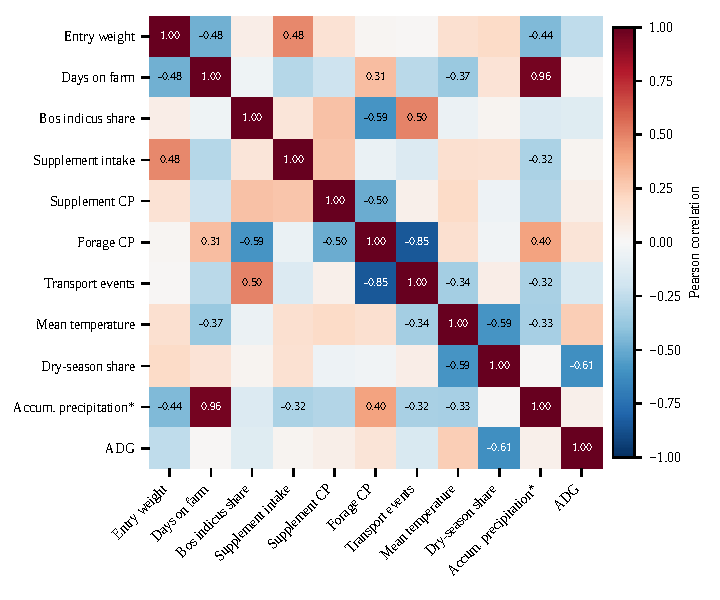
\includegraphics[width=0.75\textwidth]{figs/fig_corrmat_en.pdf}
\caption{Pearson correlations among the nine predictors, the accumulated precipitation (*, left out of the models) and ADG. Values with absolute value below 0.3 are not printed.}\label{fig:corrmat}
\end{figure}

The remaining nine predictors are listed in Table~\ref{tab:vars} with the reason for using each one.

\begin{table}[H]
\caption{Predictors.}\label{tab:vars}
\small
\begin{tabular}{>{\raggedright\arraybackslash}p{2.9cm}>{\raggedright\arraybackslash}p{4.4cm}>{\raggedright\arraybackslash}p{4.0cm}}
\hline
Variable & Description & Reason\\
\hline
Entry weight & Weight at the entry weighing (kg) & Starting point of the cycle\\
Days on farm & Days between entry and exit & Length of the period over which the gain is averaged\\
\textit{Bos indicus} share & Share of \textit{Bos indicus} by breed (50, 75 or 100\%) & Genotype affects ADG \cite{veneto}\\
Mean supplement intake & Supplement intake per day, averaged over the cycle (kg/day) & Supplementation changes the gain on pasture \cite{tambara2021}\\
Supplement CP & Crude protein of the supplement (20, 25 or 30\%) & Protein supply of the supplement\\
Forage CP & Crude protein of the forage (10.42\% in A, 10.0\% in B) & Quality of the pasture\\
Transport events & Number of transport events (1 to 3) & Transport stress\\
Mean temperature & Mean air temperature between entry and exit (\textdegree C) & Weather affects ADG \cite{ndsuweather}\\
Dry-season share & Share of the cycle between April and September & Season affects ADG \cite{tambara2021,veneto}\\
\hline
\end{tabular}
\end{table}

We defined the dry season as April to September. In the NASA POWER data for farm A, mean monthly rainfall from 2015 to 2024 was below 50~mm in those months and above 120~mm in the others. The literature gives April to September for the Zona da Mata \cite{furlong1985} and May to September for the Cerrado \cite{gomes2015estrategias}.

Table~\ref{tab:desc} gives the mean and standard deviation of the ADG, the weights and the days on farm, by farm and in total.

\begin{table}[H]
\caption{Mean and standard deviation by farm and in total.}\label{tab:desc}
\small
\setlength{\tabcolsep}{4pt}
\begin{tabular}{lcccccccc}
\hline
 & \multicolumn{2}{c}{ADG (kg/day)} & \multicolumn{2}{c}{Entry weight (kg)} & \multicolumn{2}{c}{Exit weight (kg)} & \multicolumn{2}{c}{Days on farm}\\
 & Mean & SD & Mean & SD & Mean & SD & Mean & SD\\
\hline
Farm A ($n=174$) & 0.359 & 0.087 & 178 & 46 & 315 & 48 & 390 & 195\\
Farm B ($n=71$) & 0.326 & 0.168 & 176 & 46 & 267 & 59 & 265 & 122\\
Total ($n=245$) & 0.350 & 0.117 & 177 & 46 & 301 & 55 & 354 & 186\\
\hline
\end{tabular}
\end{table}

Farm A has the higher and more homogeneous ADG. Its mean is 0.359~kg/day, ranging from 0.134 to 0.612. Farm B has a lower mean of 0.326~kg/day and a spread almost twice as large, from $-0.186$ to 0.676, and all four animals that lost weight are in B. Entry weight is similar in the two farms, with means of 178 and 176~kg and ranges of 25 to 298~kg in A and 89 to 283~kg in B. Exit weight and days on farm differ. Animals in A leave heavier, at 315 against 267~kg, and stay longer, with a mean of 390 days up to 1253 in A against 265 days up to 383 in B.

Animals in the same lot share dates, climate and management, so we also group them by lot when validating the models (Section~\ref{sec:val}). A lot is the set of animals with the same farm, entry date and exit date. There are 66 lots, 59 in A and 7 in B. Of these, 29 have a single animal, and the largest has 19.

\subsection{Exploratory data analysis}

Farm B entered 64 of its 71 animals in 2020 and the other 7 in 2021, while farm A entered between 11 and 46 animals per year from 2020 to 2025 (Fig.~\ref{fig:eda}a). ADG is skewed to the left, with a skewness of $-0.89$ (Fig.~\ref{fig:eda}b), and days on farm are longer in A (Fig.~\ref{fig:eda}c).

\begin{figure}
\centering
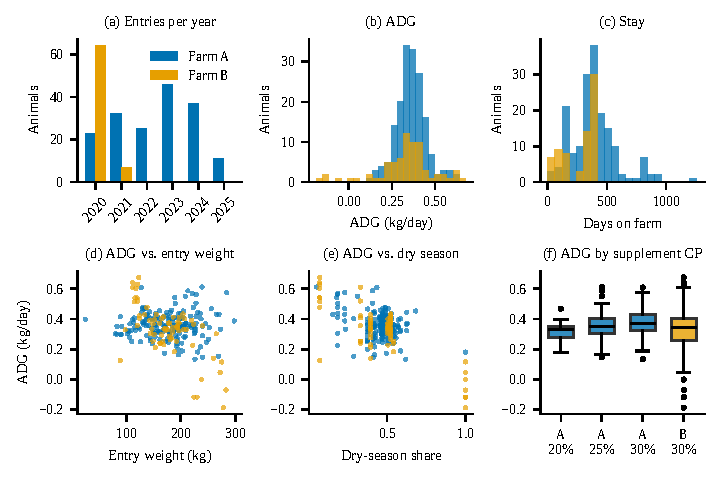
\includegraphics[width=\textwidth]{figs/fig_eda_en.pdf}
\caption{Overview of the 245 animals by farm (A in blue, B in orange): (a) entries per year; (b) distribution of ADG; (c) days on farm; (d) ADG against entry weight; (e) ADG against the dry-season share of the cycle; (f) ADG by supplement CP.}\label{fig:eda}
\end{figure}

Eight animals, seven in B and one in A, have cycles of 43 or 44 days, all in the dry season, with a mean ADG of $-0.018$~kg/day. They include the four animals with negative ADG, whose weight changes were between $-8$ and $-3$~kg over 43 days, which is compatible with weighing error in short intervals. In A the mean ADG is 0.319~kg/day with supplement CP of 20\%, 0.352 with 25\% and 0.379 with 30\% (Fig.~\ref{fig:eda}f), and every animal in B receives 30\%.

The strongest linear correlation with ADG is the dry-season share of the cycle, at $-0.61$ (Figs.~\ref{fig:corrmat} and \ref{fig:eda}e), and the eight short cycles account for part of it: without them it falls to $-0.40$. Entry weight and mean temperature come next, at $-0.25$ and $+0.25$ (Fig.~\ref{fig:eda}d). Days on farm and mean supplement intake have linear correlations close to zero, $+0.01$ and $+0.03$, which does not rule out nonlinear relations. Management variables take few values within each farm and are confounded with the farm itself, so a model can use them to tell the farms apart.

\subsection{Models}

We compared four models: linear regression, XGBoost, a DNN, and TabPFN. Linear regression is ordinary least squares on standardized variables. XGBoost \cite{chen2016xgboost} is a gradient-boosted tree ensemble, and we tuned its number of trees, maximum depth, learning rate, subsample, and minimum child weight by grid search.

The DNN is a multilayer perceptron with layers of 128, 64, 32 and 16 units (12,641 parameters), batch normalization \cite{ioffe2015batchnorm} and ReLU after each layer, a linear output and no dropout. We trained it with Adam \cite{kingma2015adam}, with a learning rate of 0.01, a weight decay of $10^{-4}$, batches of 32 and the Huber loss \cite{huber1964robust}. We held out 25\% of the training set to monitor the Huber loss, and variables and target were standardized with the statistics of the remaining 75\%. The learning rate was halved after 8 epochs without improvement on the held-out loss. Training stopped after 60 epochs without improvement or at 300 epochs, and we kept the weights with the lowest held-out loss. The hidden layers, dropout, learning rate, batch normalization and weight decay were chosen by grid search and then frozen. The reported DNN is the mean of five networks with different seeds, implemented in PyTorch \cite{pytorch2023}.

We searched the values in Table~\ref{tab:grid}, which gives 48 combinations for XGBoost (2 $\times$ 3 $\times$ 2 $\times$ 2 $\times$ 2) and 72 for the DNN (3 $\times$ 2 $\times$ 3 $\times$ 2 $\times$ 2). Each combination was evaluated on the five farm-stratified folds of Section~\ref{sec:val}, with a single network per fold for the DNN, and we selected the one with the highest mean $R^2$ over the folds. The selected XGBoost setting has 200 trees, depth 3, learning rate 0.1, subsample 0.8, and minimum child weight 1.

\begin{table}[H]
\caption{Grid search: values searched for each hyperparameter and the configuration selected.}\label{tab:grid}
\small
\begin{tabular}{>{\raggedright\arraybackslash}p{1.8cm}>{\raggedright\arraybackslash}p{3.4cm}>{\raggedright\arraybackslash}p{3.8cm}>{\raggedright\arraybackslash}p{2.4cm}}
\hline
Model & Hyperparameter & Values & Selected\\
\hline
XGBoost & Number of trees & 200, 400 & 200\\
 & Maximum depth & 2, 3, 4 & 3\\
 & Learning rate & 0.03, 0.1 & 0.1\\
 & Subsample & 0.8, 1 & 0.8\\
 & Minimum child weight & 1, 5 & 1\\
\hline
DNN & Hidden layers & (64, 32); (128, 64, 32); (128, 64, 32, 16) & (128, 64, 32, 16)\\
 & Dropout & 0, 0.1 & 0\\
 & Learning rate & 0.003, 0.005, 0.01 & 0.01\\
 & Batch normalization & off, on & on\\
 & Weight decay & 0, $10^{-4}$ & $10^{-4}$\\
\hline
\end{tabular}
\end{table}

TabPFN is a transformer pre-trained on millions of synthetic tabular data sets \cite{hollmann2025tabpfn}. It does not update its weights on a new data set: the training animals are given as context and the test animals are predicted in a single forward pass. We used the default \texttt{TabPFNRegressor} of the \texttt{tabpfn} package (version 9.0.0, model 3.5 \cite{jager2026tabpfn35}), with unscaled variables and no tuning. Its 5\% and 95\% quantiles give a 90\% prediction interval. Linear regression and the validation routines use scikit-learn \cite{pedregosa2011sklearn}.

\subsection{Validation protocol}\label{sec:val}

We used three schemes. Wherever variables were scaled, the scaling was fitted on the training animals only.

\textit{Farm-stratified cross-validation.} Five disjoint folds, each with 49 test animals (35 from A and 14 from B in four folds, 34 and 15 in the other), so every animal is tested once.

\textit{Lot-grouped cross-validation.} Five folds in which no lot is split between training and test. Lots are sorted from the largest to the smallest, with lots of the same size in random order, and each one goes to the fold that has the fewest animals so far. This keeps the folds near 49 animals. The folds are not stratified by farm.

\textit{Train on one farm, test on the other.} We train on A and test on B, and the reverse, once each and without refitting the hyperparameters.

The first two schemes were repeated 10 times with different random partitions, and all models use the same nine predictors and the same partitions. We report the mean absolute error (MAE, in kg/day) and the coefficient of determination $R^2$ per fold, and the $R^2$ of the predictions pooled over the five folds of each repetition. To compare models we used the paired differences in MAE per fold with the corrected resampled $t$ test of Nadeau and Bengio \cite{nadeau2003}, and the Holm correction \cite{holm1979} over the six pairs of models in each scheme.

The hyperparameters of the DNN and XGBoost were chosen on the folds of the first scheme, which favors these two models. To measure that bias, we also ran nested validation: the same grids were searched inside each training set, with three inner folds stratified by farm, and the selected configuration was evaluated on the outer fold. This was done for the first two repetitions of the farm-stratified scheme. TabPFN and linear regression are not tuned.

\subsection{Interpretation}

We computed SHAP values \cite{lundberg2017shap} for TabPFN with the model-agnostic \texttt{KernelExplainer}, using 20 background samples, on the model fitted to all 245 animals. We report the mean absolute value per variable.

\section{Results and Discussion}

\subsection{Comparison under repeated cross-validation}

Table~\ref{tab:cv} and Fig.~\ref{fig:cv} give the results of the 10 repetitions of 5-fold cross-validation. With folds stratified by farm, the ranking by MAE is TabPFN (0.0149~kg/day), DNN (0.0290), XGBoost (0.0520) and linear regression (0.0634). All six paired differences are significant after the Holm correction (Table~\ref{tab:tests}). The difference between TabPFN and the DNN is 0.014~kg/day, about half the DNN error. The $R^2$ computed on the pooled out-of-fold predictions is 0.887 for TabPFN and 0.827 for the DNN, against 0.575 for XGBoost and 0.475 for linear regression.

\begin{table}
\caption{Repeated cross-validation (10 repetitions of 5 folds). MAE in kg/day: mean over folds (standard deviation over folds); $R^2$ on the pooled out-of-fold predictions.}\label{tab:cv}
\begin{tabular}{p{2.4cm}p{2.6cm}p{1.6cm}p{2.6cm}p{1.6cm}}
\hline
 & \multicolumn{2}{c}{Farm-stratified} & \multicolumn{2}{c}{Lot-grouped}\\
Model & MAE & $R^2$ & MAE & $R^2$\\
\hline
Linear regression & 0.0634 (0.0076) & 0.475 & 0.0725 (0.0120) & 0.333\\
XGBoost & 0.0520 (0.0083) & 0.575 & 0.0607 (0.0205) & 0.404\\
DNN & 0.0290 (0.0060) & 0.827 & 0.0356 (0.0150) & 0.709\\
TabPFN & 0.0149 (0.0051) & 0.887 & 0.0242 (0.0183) & 0.735\\
\hline
\end{tabular}
\end{table}

\begin{figure}
\centering
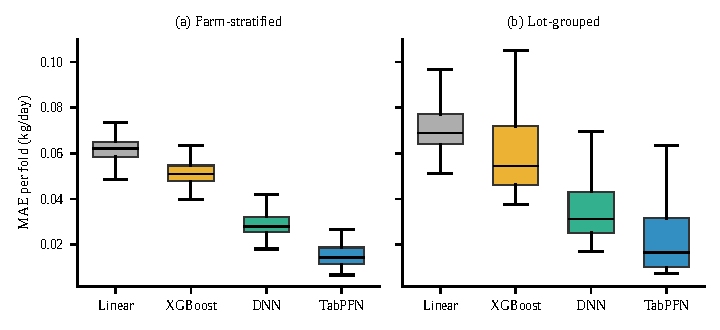
\includegraphics[width=\textwidth]{figs/fig_cv_en.pdf}
\caption{MAE per fold over 10 repetitions of 5-fold cross-validation: (a) folds stratified by farm; (b) folds grouped by lot.}\label{fig:cv}
\end{figure}

\begin{table}
\caption{Paired comparisons of MAE (mean difference in kg/day, first model minus second; Holm-adjusted $p$ values).}\label{tab:tests}
\begin{tabular}{p{4.0cm}p{1.8cm}p{1.8cm}p{1.8cm}p{1.8cm}}
\hline
 & \multicolumn{2}{c}{Farm-stratified} & \multicolumn{2}{c}{Lot-grouped}\\
Pair & Diff. & $p$ & Diff. & $p$\\
\hline
Linear $-$ XGBoost & 0.011 & 0.002 & 0.012 & 0.095\\
Linear $-$ DNN & 0.034 & $<$0.001 & 0.037 & $<$0.001\\
Linear $-$ TabPFN & 0.049 & $<$0.001 & 0.048 & $<$0.001\\
XGBoost $-$ DNN & 0.023 & $<$0.001 & 0.025 & $<$0.001\\
XGBoost $-$ TabPFN & 0.037 & $<$0.001 & 0.036 & $<$0.001\\
DNN $-$ TabPFN & 0.014 & $<$0.001 & 0.011 & 0.068\\
\hline
\end{tabular}
\end{table}

Grouping the folds by lot raises the error of every model, and by different amounts. Linear regression goes from 0.0634 to 0.0725 and its fold-level $R^2$ falls from 0.424 to 0.059. XGBoost goes from 0.0520 to 0.0607. The DNN and TabPFN lose less in $R^2$ (0.827 to 0.709 and 0.887 to 0.735), but their errors rise by 23\% and 62\%. Animals of the same lot share dates, and so the mean temperature and the dry-season share work almost as lot identifiers when lots are split between training and test. A model may use them to recognize the lot instead of learning how climate affects gain. The lot-grouped scheme removes this shortcut, and its results are the more realistic estimate for a new lot on a known farm. Under it the DNN and TabPFN are still well ahead of XGBoost and linear regression, but the 0.011~kg/day gap between them is no longer significant (adjusted $p=0.068$), and XGBoost and linear regression cannot be separated either ($p=0.095$). The fold-level standard deviation of TabPFN also grows from 0.0051 to 0.0183, so its advantage depends on which lots end up in the test fold.

The 90\% prediction intervals of TabPFN covered 96.8\% of the test animals under the farm-stratified scheme (mean width 0.065~kg/day) and 95.1\% under the lot-grouped one (0.104). They are conservative, wider than needed for the nominal level, and widen when lots are held out. These coverages describe cross-validation only, not new farms.

\subsection{Selection bias}

The grids of the DNN and XGBoost were searched on the same folds used for evaluation. In the nested validation, the MAE of the DNN rose from 0.0291 to 0.0314~kg/day and its $R^2$ fell from 0.804 to 0.775. For XGBoost the MAE rose from 0.0527 to 0.0575 and $R^2$ from 0.509 to 0.451. The bias is small compared with the gap to TabPFN, which has no tuned hyperparameters, and the ranking does not change. The DNN selected the same configuration (no dropout, learning rate 0.01, batch normalization, weight decay $10^{-4}$) in 8 of 10 outer folds, and only its architecture varied. XGBoost chose 8 different configurations in 10 folds. We kept the frozen configuration as the main result.

\subsection{Transfer between farms}

When we train on one farm and test on the other, the picture changes (Table~\ref{tab:lopo}). Testing on B, TabPFN reaches $R^2=0.48$, the DNN 0.35 and XGBoost 0.29, while linear regression gives $-1.61$. Testing on A, every model is worse than predicting the training mean ($R^2$ from $-0.74$ for XGBoost to $-71.0$ for linear regression), and the DNN and TabPFN degrade the most ($-49.3$ and $-29.8$). XGBoost is the most stable in this scheme. A is larger (174 animals), has cycles up to 1253 days and several supplement levels, while B has 71 animals with cycles of at most 383 days. A model trained on B never sees most of the range it is asked to predict, and flexible models probably extrapolate from it badly. Two farms cannot tell farm effects from the limits of the training range, and this scheme was run only once, without repetitions or intervals.

\begin{table}
\caption{$R^2$ when training on one farm and testing on the other (single run).}\label{tab:lopo}
\begin{tabular}{p{4.0cm}p{3.0cm}p{3.0cm}}
\hline
Model & Test on B & Test on A\\
\hline
Linear regression & $-1.61$ & $-71.0$\\
XGBoost & 0.29 & $-0.74$\\
DNN & 0.35 & $-49.3$\\
TabPFN & 0.48 & $-29.8$\\
\hline
\end{tabular}
\end{table}

\subsection{Variable importance}

Entry weight (mean $|$SHAP$|$ 0.171~kg/day), mean supplement intake (0.136) and days on farm (0.093) account for most of the attributions of TabPFN (Fig.~\ref{fig:shap}). The dry-season share follows with 0.023, and the other five variables stay below 0.01. That entry weight and supplement intake matter most is plausible for cattle growing on pasture. The two variables correlated at $-0.85$, forage CP and transport events, have low importance (0.006 and 0.004), so their collinearity does not change this reading. Forage CP takes only two values, one per farm, and cannot be told apart from the farm itself. The SHAP values were computed on a model fitted to all animals and carry no causal interpretation.

\begin{figure}
\centering
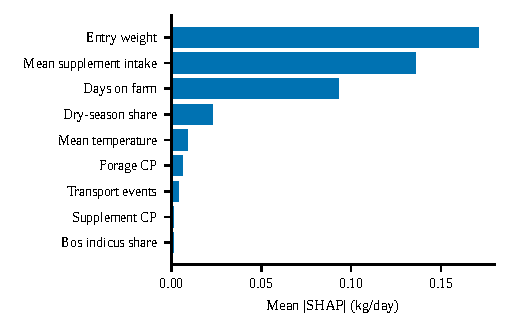
\includegraphics[width=0.7\textwidth]{figs/fig_shap_en.pdf}
\caption{Mean absolute SHAP value of each variable for TabPFN fitted to all 245 animals.}\label{fig:shap}
\end{figure}

\subsection{Limitations}

The data set has 245 females from two farms in one region, so the results do not cover males, other regions or other management systems. Several variables are constant within a farm. The 10 repetitions reuse the same animals, so the corrected $t$ test is an approximation. The farm-to-farm results come from one run. 29 of the 66 lots have one animal, and the eight short cycles contribute negative gains that may be weighing error.

\section{Conclusion}

Under repeated cross-validation, TabPFN predicted the ADG of the 245 cattle with the lowest error, followed by a tuned DNN, XGBoost and linear regression, and nested validation showed that tuning bias does not explain the ranking. When lots are held out the error of every model rises and the difference between TabPFN and the DNN is no longer significant. Models trained on one farm did not predict the other farm reliably. For practical use, a model should be validated by lot and by farm before it supports decisions, and more farms are the next step to test whether the ranking holds.

\begin{credits}
\subsubsection{\ackname} [Acknowledgments and funding statement: to be completed.]

\subsubsection{\discintname}
The authors have no competing interests to declare that are relevant to the content of this article.

\subsubsection{Use of generative AI} A generative AI assistant was used to help draft and edit the code for the experiments and the text of this manuscript. The authors reviewed the output and take responsibility for the content.
\end{credits}
%
% ---- Bibliography ----
%
\bibliographystyle{splncs04}
\bibliography{refs}
\end{document}
